\chapter{Hyökkäyksiltä suojautuminen\label{discussion}}

Tässä kappaleessa käydään läpi erilaisia puolustusmenetelmiä NLP-hyökkäyksiä vastaan. NLP-hyökkäykset voidaan torjua korkean tason abstraktiolla, suurella yleisrasituksella, sekä alemman tason abstraktiolla, pienemmällä yleisrasituksella. Ensiksi esitellään korkean tason abstraktion OCR-puolustus, sitten kuvaillaan alemman tason abstraktion suorituskeskeinen puolustautuminen.

\section{OCR-puolustus}
OCR-metodia (eng. OCR, Optical character recognition), eli tekstintunnistusta on käytetty esimerkiksi printatun, skannatun tai käsinkirjoitetun tekstin muuntamiseen muokattavaksi tekstiksi. Joskus tekstint tunnistaminen on vaikeata johtuen esimerkiksi tekstin eri koista, tyyleistä, suuntauksesta tai monimutkaisesta tekstin taustasta. Esimerkiksi nolla-merkki ''0'' ja aakkonen ''o'' voivat olla jollekkin OCR-työkalulle vaikeita erottaa toisistaan. Kyseistä virhelukua havainnollistetaan kuvassa 4.1 ja 4.2. Eri OCR-työkalut saavuttavat tekstintunnistuksen eri tavoilla, mutta esimerkiksi avoimen lähdekoodin OCR-työkalu Tesseractilla on seuraavat vaiheet tekstintunnistukseen kuvasta: (1) kuvan muuntaminen binäärikuviksi, (2) merkkien ääriviivojen tunnistamiset, (3) merkkien ääriviivojen tunnistaminen sanoiksi, (4) sanat tunnistetaan kahteen kertaan, jonka jälkeen teksti on tunnistettu kuvasta. Kuva 4.3 havainnollistaa edelläkuvattua Tesseractin tekstintunnistusprosessia \citep{tesseractocr}.

\begin{figure}[t]
  
\includegraphics[scale=0.6]{figures/moonshine.png}
  \caption{Tekstitunnistettava kuva \citep{tesseractocr}}
\end{figure}

\begin{figure}[t]
  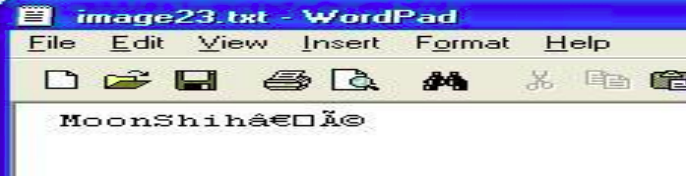
\includegraphics[scale=0.6]{figures/failmoonshine.png}
  \caption{Tesseract epäonnistuu tunnistamaan ylätekstin ''Effect'' kuvasta \citep{tesseractocr}}
\end{figure}

OCR-puolustuksen läpikäynnin jälkeen voidaan huomata metodin eliminoivan huomattavan monta NLP-hyökkäystä. Näkymättömät merkit, poistatukset sekä uudelleenjärjestelymerkit poistuvat kokonaan tekstintunnistuksen jälkeen tuotetusta tekstistä, koska kyseiset merkit eivät ihmissilmällekkään näkyisi. Roskapostisuodatuksen -ja sensuurin ohituksen lisäksi OCR-puolustus alisuoriutuu eräällä toisellakin osa-alueella.

\begin{figure}[t]
  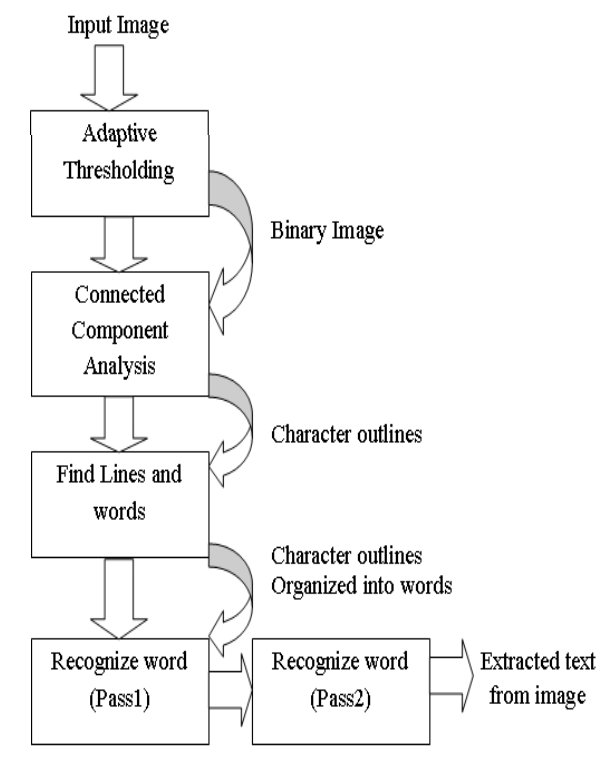
\includegraphics[scale=0.4]{figures/tesseract.png}
  \caption{Tesseractin tekstintunnistuksen vaiheet \citep{tesseractocr}}
\end{figure}

Tekstintunnituksen avulla epäselvyydet tekstin aidosta luonteesta voidaan hahmontaa uudelleen tulkitsemalla aineisto uudestaan visuaalisesti. Tämä menetelmä lisää yleisrasitusta huomattavasti riippuen käyttötarkoituksesta, mutta poistaa pahantahtoiset merkit ilman NLP-luokittimen uudelleenkoulutusta. \citep{boucher2021bad}

\section{Suorituskykykeskeinen puolustus}
Keskitymme seuraavaksi näkymättömiin merkkeihin, -homoglyfeihin, \-uudelleenjärjestelyihin -ja poistatuksiin perustuvien hyökkyksien puolustamiseen. Osat suorituskykykeskeisistä puolustusmenetelmistä ovat kuitenkin laskennallisesti kalliita, eivätkä koneoppimismallin ulkoistaneet yritykset yleensä pysty kustantamaan kyseisiä metodeita \citep{https://doi.org/10.48550/arxiv.1911.07399}.

Näkymättöimen merkkein tapauksessa, tietyt näkymättömät merkit voidaan poistaa suoraan syötteestä. Mikäli sovelluksessa näitä merkkejä ei voida poistaa, voidaan ne korvata \textit{ei-}\texttt{<unk>} upotuksilla. Korvaus tapahtuu lähdekielisanakirjassa, jonne kuvataan tuntematon merkki ''ei-tuntemattomaksi tokeniksi''. Näin tuntemattomat merkit eivät voi häiritä ladontaa merkeillä, joista ladontamoottori ei ole aivan varma. Homoglyfihyökkäysten torjuminen OCR-menetelmällä on ymmärrettävästi vaikeampaa verrattuina muihin merkkeihin. Paras keino torjua tällaisia hyökkäyksiä olisi kuvata osa homoglyfeistä niiden yleisemmin tunnettuihin vastineisiin. NLP-luokittimen ylläpitäjä joutuu tekemään tässä siis suurimman työn. Uudelleenjärjestelyhyökkäykset voidaan torjua riisumalla kaksisuuntais-ohjausmerkit\\syötteestä, varoittamalla käyttäjää kaksisuuntais-ohjausmerkkien ilmestyessä syötteeseen tai käyttämällä kaksisuuntais-algoritmia halutun syötteen selvittämiseen. Puolustusmenetelmän valinta riippuu kontekstista, sillä esimerkiksi latinaa tai arabiaa kirjoittaessa ohjelma toimisi väärin pakottamalla käyttäjän syötteestä pois kaksisuuntais-ohjausmerkin \texttt{U+200F}. Poistatukset yleensä havaitaan NLP-luokittimien ulkopuolella syötteen annon alkuvaiheessa. NLP-luokittimen tasolla tähän tarvitsee harvemmin puuttua ja käyttäjälle voidaan pahimmassa tapauksessa lähettää varoitus poistatusmerkkien olemassaolosta syötteessä. On silti tärkeää tiedostaa poistatuksien puolustus, mikäli käyttöjärjestelmä unohtaa puuttua kyseiseen hyökkäystyyppiin. \citep{boucher2021bad}

Roskapostisuodattimeen -ja sensuurin ohitukseen kohdistuvat hyökkäykset voidaan yrittää torjua muun muassa DNE-metodilla (eng. Dirichlet Neighborhood Ensemble). Metodissa korvataan virtuaalisten lauseiden sanoja näiden synonyymeillä. Tämän jälkeen puolustava NLP-luokitin koulutetaan kyseisiä lauseita vastaan. Metodin tarkoituksena on siis puolustautua synonyymin korvausta vastaan, joka esiteltiin alikappaleessa 2.1, Roskapostisuodatuksen ohitus \citep{dnedefense}.